\section{Engineering Challenges}
Research challenges such as static analysis of exit points and veritesting in a multi-threaded context need to be solved for integrating veritesting with any bytecode-level symbolic execution engine.
%
Symbolic PathFinder is a popular Java bytecode-level symbolic execution tool.
%
It has been used to find bugs in flight software~\cite{pasareanu2008}, to test large web applications~\cite{fujitsu}, and for testing Android apps~\cite{android_spf}.
%
It has also been extended for parallel symbolic execution~\cite{parallel}, and for load testing~\cite{load_testing_spf}
%Talk about the engineering challenges we face when implementing veritesting with Symbolic PathFinder
%
Given the large and diverse set of applications that stand to benefit from integrating veritesting with SPF, we discuss here the engineering challenges expected with such an integration.

\subsection{Shared Sub-expressions} 
%Sharing implementation needs to be fixed. Show this using the TestSharing example
Consider the code shown in Listing~\ref{lst:sharing}.
%
\lstinputlisting[caption={An example with an increasing formula size with every loop iteration}, 
label={lst:sharing}]{code_samples/TestSharing.java}
%
The function \textit{testSharing} adds the value of \textit{x} to itself in every loop iteration on line 3 of Listing~\ref{lst:sharing}.
%
The number of loop iterations is controlled by a user-supplied value for \textit{bound}.
%
On line 4, the code branches on the value of the value of \textit{x}.
%
We symbolically executed the \textit{testSharing} method with \textit{x} set to be symbolic and \textit{bound} set to be a concrete value.
%
We set the minimum and maximum symbolic integer values to be -100 and 100 respectively.
%
We increased the value of \textit{bound} from 1 to 29 and recorded the time taken and maximum memory used for complete path coverage.
%
Figure~\ref{fig:sharing_time} shows the trend seen for increasing values of \textit{bound}.
%
\begin{figure}[]
\caption{Time required for covering paths in Listing~\ref{lst:sharing} with increasing values for \textit{bound}}
\label{fig:sharing_time}
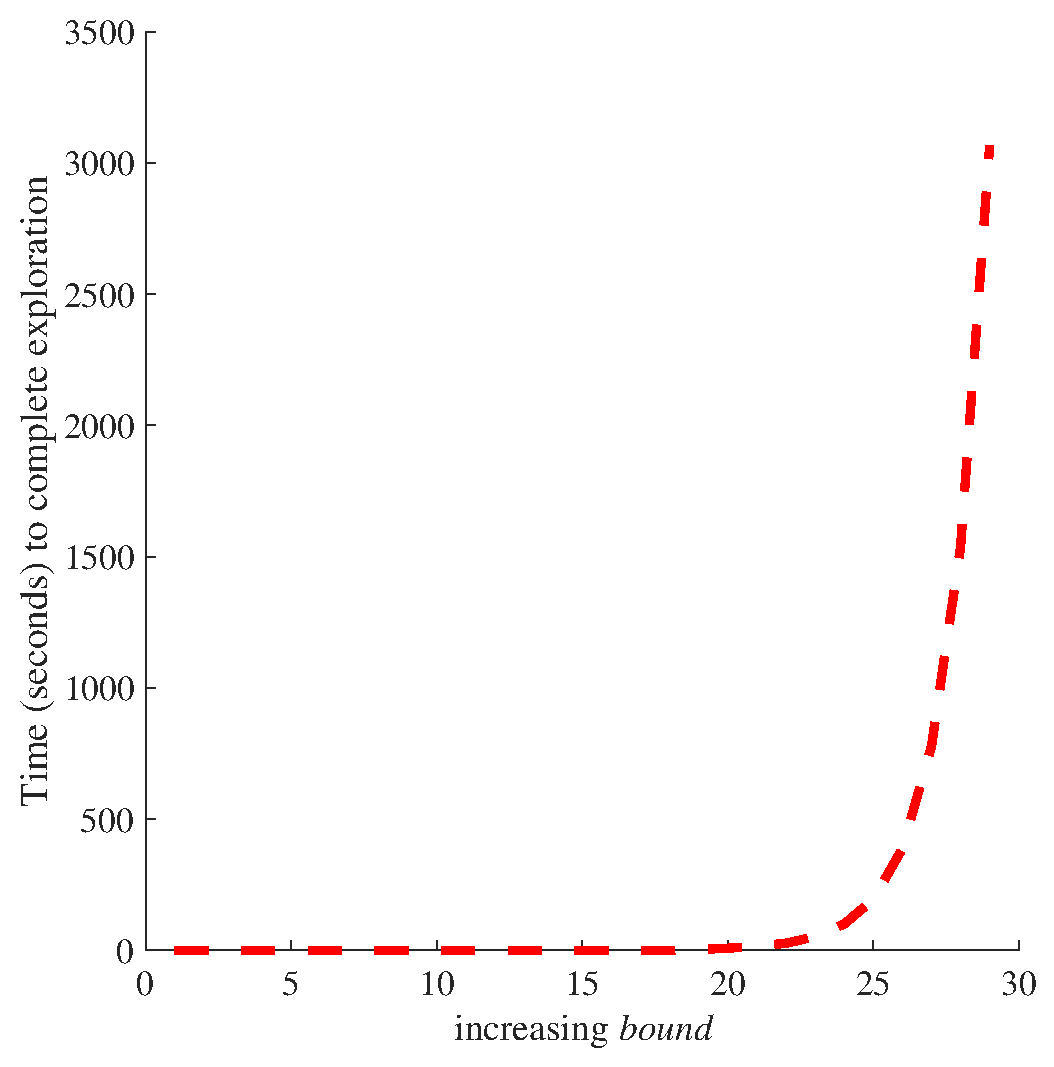
\includegraphics[width=\columnwidth]{figures/sharing_time}
\end{figure}
%
Figure~\ref{fig:sharing_time} shows that the running time remains constant until the value for \textit{bound} is 18, and then starts to rise exponentially.

\subsection{Complex Expressions}
Engineering issue \#2: Need to have complex expressions, talk about how Comparators cannot be used anywhere below the top-level operator

\subsection{Intermediate variables}
Engineering issue \#3: Nice to introduce intermediate variables
